\section{Docker Daemon Attacks}\label{attacker-model:daemon-attacks}
In a Docker daemon attack, an attacker has access to a host with Docker installed on it. The attacker might be able access sensitive and privileged information by interacting with the Docker daemon or by reading Docker configuration files. Unlike container escapes, the attacker does not attack Docker or the isolation that Docker creates directly, but uses Docker to perform malicious actions.

\medskip

This is attack is shown in \autoref{fig:docker-daemon-attack}.

\begin{figure}[ht]
    \centering
    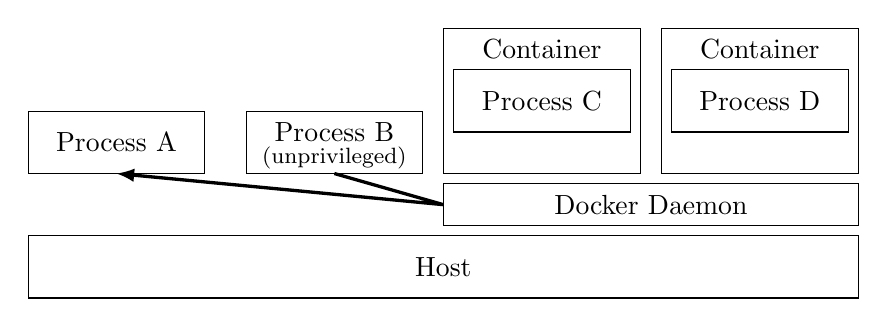
\begin{tikzpicture}[x=0.75pt,y=0.75pt,yscale=-1,xscale=1]
        % Host Rectangle
        \draw (0,100) -- (400,100) -- (400,130) -- (0,130) -- cycle ;
        \draw (200, 115) node {Host};

        %Docker Daemon Rectangle
        \draw (200,75) -- (400,75) -- (400,95) -- (200,95) -- cycle ;
        \draw (300,85) node {Docker Daemon};

        % Process A Rectangle
        \draw (0,40) -- (85,40) -- (85,70) -- (0,70) -- cycle ;
        \draw (42.5,55) node {Process A};

        % Process B Rectangle
        \draw (105,40) -- (190,40) -- (190,70) -- (105,70) -- cycle ;
        \draw (147.5,50) node {Process B};
        \draw (147.5,62.5) node {{\footnotesize (unprivileged)}};

        %Container Process C Rectangle
        \draw (200,0) -- (295,0) -- (295,70) -- (200,70) -- cycle ;
        \draw (247.5,10) node {Container};

        %% Process C Rectangle
        \draw (205,20) -- (290,20) -- (290,50) -- (205,50) -- cycle ;
        \draw (247.5,35) node {Process C};

        %Container Process D Rectangle
        \draw (305,0) -- (400,0) -- (400,70) -- (305,70) -- cycle ;
        \draw (352.5,10) node {Container};

        %% Process D Rectangle
        \draw (310,20) -- (395,20) -- (395,50) -- (310,50) -- cycle ;
        \draw (352.5,35) node {Process D};

        % Line
        \draw [-latex, very thick] (147.5,70) -- (200,85) -- (42.5,70);
    \end{tikzpicture}
    \caption{}\label{fig:docker-daemon-attack}
    \medskip
    \small
    An unprivileged process B accessing privileged data (in the image process A) using the Docker daemon.
\end{figure}

Because Docker needs a lot of kernel features to function properly, the Docker daemon needs to run as \lstinline{root}. This makes it a very interesting target, because vulnerabilities that allow an attacker to maliciously control the Docker daemon, allow the attacker to perform actions as \lstinline{root}.
